\section{Methodology}
The \acrshort{daq} system is implemented using an Arduino UNO R3 with a LM35 temperature sensor connected to it, as shown in Fig~\ref{fig:arduino_daq}.

\begin{figure}[H]
    \centering
    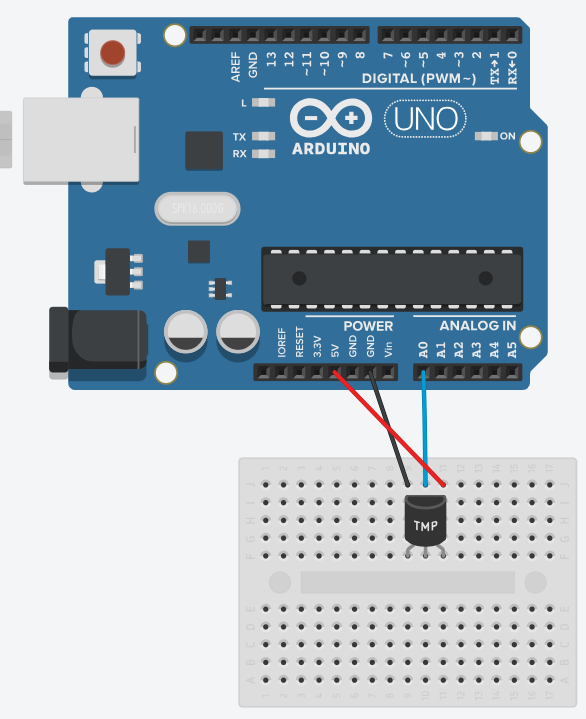
\includegraphics[width=0.6\linewidth]{figures/arduino_daq.png}
    \caption{Diagram representing the Arduino DAQ system}
~\label{fig:arduino_daq}
\end{figure}

The Arduino \acrshort{daq} system performs two primary functions. Initially, it measures the ambient temperature in millivolts ($mV$), which is then converted to Celcius degrees using a LM35.h library by Steven Wilmouth. The resulting temperature value is then supplied to the the Kalman filter algorithm. Secondly, it reads a digital signal indicating the status of the heating system, whether it is activate or deactivated that is used as the excitation function. \\

To take care of common matrix and vector mathematical operations like additon, substraction, multiplication, transposing, invertion and other, some miscelanious functions were coded, as shown below:

\lstinputlisting[language=C++]{codes/MathMatrix.hpp}

Kalman filter was implemented using Object-Oriented Programming. The class consists of three two main methods. For \textit{set\_params} method, constants like $H$, $R$, $\Gamma$, $\Phi$ and $Q$ are passed and are set as class attributes to use it later during prediction stage. The \textit{predict} method is used to apply the Kalamn algorithm. It takes the value of $x(k)$, $P(k)$, $y(t)$, and $u(k)$ to make the prediction of $x(k+1)$ and $P(k+1)$. The code can be seen below.

\lstinputlisting[language=C++]{codes/KalmanFilter.hpp}

Additionally, for the simulation, the following parameters are used:

\begin{itemize}
    \item $\tau$: the time constant of the system is set to 20s.

    \item $K_{p}$: the gain of the system is set to 0.5.

    \item $\sigma$: the standard deviation of the Gaussian white noise is set to 0.08.

    \item $\Delta t$: the sampling time is set to 1 seconds.
\end{itemize}

The parameters for the filter were computed as:

\begin{equation}
    R = \sigma^2 = (0.08)^2 = 0.0064
\end{equation}

\begin{equation}
    \phi(k) = e^{a \cdot \Delta t} = e^{-0.05 \cdot 1} = 0.6065
\end{equation}

\begin{equation}
    \Gamma(k) = \frac{0.025}{-0.05} \left( e^{-0.05 \cdot 1} - 1\right) = 0.1967
\end{equation}

The code used to test the Arduino \acrshort{daq} system, is shown below:

\lstinputlisting[language=C++]{codes/Daq.ino}


